%% 
%% Copyright 2007-2020 Elsevier Ltd
%% 
%% This file is part of the 'Elsarticle Bundle'.
%% ---------------------------------------------
%% 
%% It may be distributed under the conditions of the LaTeX Project Public
%% License, either version 1.2 of this license or (at your option) any
%% later version.  The latest version of this license is in
%%    http://www.latex-project.org/lppl.txt
%% and version 1.2 or later is part of all distributions of LaTeX
%% version 1999/12/01 or later.
%% 
%% The list of all files belonging to the 'Elsarticle Bundle' is
%% given in the file `manifest.txt'.
%% 

%% Template article for Elsevier's document class `elsarticle'
%% with numbered style bibliographic references
%% SP 2008/03/01
%%
%% 
%%
%% $Id: elsarticle-template-num.tex 190 2020-11-23 11:12:32Z rishi $
%%
%%
\documentclass[preprint,12pt]{elsarticle}

%% Use the option review to obtain double line spacing
%% \documentclass[authoryear,preprint,review,12pt]{elsarticle}

%% Use the options 1p,twocolumn; 3p; 3p,twocolumn; 5p; or 5p,twocolumn
%% for a journal layout:
%% \documentclass[final,1p,times]{elsarticle}
%% \documentclass[final,1p,times,twocolumn]{elsarticle}
%% \documentclass[final,3p,times]{elsarticle}
%% \documentclass[final,3p,times,twocolumn]{elsarticle}
%% \documentclass[final,5p,times]{elsarticle}
%% \documentclass[final,5p,times,twocolumn]{elsarticle}

%% For including figures, graphicx.sty has been loaded in
%% elsarticle.cls. If you prefer to use the old commands
%% please give \usepackage{epsfig}

%% The amssymb package provides various useful mathematical symbols
\usepackage{amssymb}
\usepackage{amsmath}
\usepackage{acronym}
%% The amsthm package provides extended theorem environments
%% \usepackage{amsthm}

%% The lineno packages adds line numbers. Start line numbering with
%% \begin{linenumbers}, end it with \end{linenumbers}. Or switch it on
%% for the whole article with \linenumbers.
%% \usepackage{lineno}

\journal{Nuclear Engineering and Technology}

\begin{document}

\begin{frontmatter}

%% Title, authors and addresses

%% use the tnoteref command within \title for footnotes;
%% use the tnotetext command for theassociated footnote;
%% use the fnref command within \author or \address for footnotes;
%% use the fntext command for theassociated footnote;
%% use the corref command within \author for corresponding author footnotes;
%% use the cortext command for theassociated footnote;
%% use the ead command for the email address,
%% and the form \ead[url] for the home page:
%% \title{Title\tnoteref{label1}}
%% \tnotetext[label1]{}
%% \author{Name\corref{cor1}\fnref{label2}}
%% \ead{email address}
%% \ead[url]{home page}
%% \fntext[label2]{}
%% \cortext[cor1]{}
%% \affiliation{organization={},
%%             addressline={},
%%             city={},
%%             postcode={},
%%             state={},
%%             country={}}
%% \fntext[label3]{}

\title{Technical Note: Measurement of nuclear fuel assembly's bow from visual inspection's video record}

%% use optional labels to link authors explicitly to addresses:
%% \author[label1,label2]{}
%% \affiliation[label1]{organization={},
%%             addressline={},
%%             city={},
%%             postcode={},
%%             state={},
%%             country={}}
%%
%% \affiliation[label2]{organization={},
%%             addressline={},
%%             city={},
%%             postcode={},
%%             state={},
%%             country={}}

\author[profinit]{Du\v{s}an Pla\v{s}ienka}

\affiliation[profinit]{
    organization={Profinit, s.r.o.},
    addressline={Tychonova 2},
    city={Prague},
    postcode={16000},
    country={Czechia}
}

\author[utia,cvr]{Jaroslav Knotek}

\affiliation[utia]{organization={Institute of Information Theory and Automation of the CAS},%Department and Organization
            addressline={Pod Vod\unexpanded{á}renskou V\unexpanded{\v{e}}\unexpanded{\v{z}}\unexpanded{\'{i}}},
            city={Prague},
            postcode={18208},
            country={Czechia}
            }

\affiliation[inst2]{organization={Research Centre \unexpanded{\v{R}}e\unexpanded{\v{z}}},%Department and Organization
            addressline={Hlavn\unexpanded{\'{i}} 130}, 
            city={Husinec},
            postcode={25068},
            country={Czechia}}

\author[cvr]{Marcin Kope\'{c}}
\author[cvr]{Martina Mal\'{a}}
\author[utia,cvr]{Jan Bla\v{z}ek}

\begin{abstract}
%% Text of abstract
The bow of the nuclear fuel assembly is a well-known phenomenon. One of the vital criteria during the history of nuclear fuel development has been fuel assembly's mechanical stability. Once present, the fuel assembly bow can lead to safety issues like excessive water gap and power redistribution or even incomplete rod insertion (IRI). The extensive bow can result in assembly handling and loading problems. This is why the fuel assembly's bow is one of the most often controlled geometrical factors during periodic fuel inspections for VVER when compared e.g. to on-site fuel rod gap measurements or other instrumental measurements performed on-site.
Our proposed screening method uses existing video records for fuel inspection. We establish video frames normalization and aggregation for the purposes of bow measurement. The whole process is done by digital image processing algorithms which analyze rotations of video frames, extract angles whose source is the fuel set torsion, and reconstruct torsion schema.
This approach provides results comparable to the commonly utilized method. We tested this new approach in real operation on 19 fuel assemblies with different campaign numbers and designs, where the average deviation from other methods was less than 2 \% on average.
Due to the fact, that the method has not yet been validated during full scale measurements of the fuel inspection, the preliminary results stand for that we recommend this method as a complementary part of standard bow measurement procedures to increase measurement robustness, lower time consumption and preserve or increase accuracy. After completed validation it is expected that the proposed method allows standalone fuel assembly bow measurements. 
\end{abstract}

%%Research highlights
\begin{highlights}
\item Novel method for fuel assembly bow and twist measurements 
\item Evaluation time is several times shorter
\end{highlights}


\begin{keyword}
fuel assembly \sep assembly quality \sep assembly bow \sep image processing
\end{keyword}

\end{frontmatter}

%% \linenumbers

\section{Introduction}

Working inside the nuclear reactor, the \ac{FA} undergo dimensional changes from campaign to campaign. The nuclear reactors' environment induces those changes due to e.g. lateral coolant flow, local power disturbances, gradients of temperatures combined with irradiation and in some cases also mechanical interaction between the assemblies in the core. The whole fuel assemblies' deformations can lead to handling problems resulting in safety-related issues like the \ac{IRI} \cite{Andersson2005}.  In this way, periodic fuel assemblies' inspections are crucial to compare the design behavior model with the real fuel condition and to verify if the fuel meets the safety criteria \cite{Aleshin2018}, \cite{Schrire2014}. Data from fuel inspection and compliance with the fuel design also serve as the input for calculation codes used, e.g. for safety analyses. In this way, data is valuable for both fuel vendors and utilities.

\begin{figure}
    \centering
    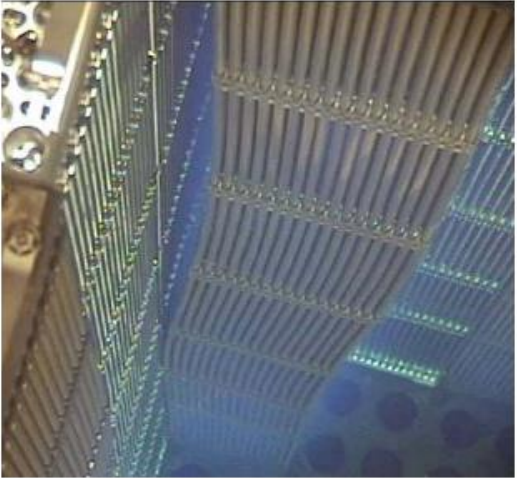
\includegraphics[width=\linewidth]{FAbowed.PNG}
    \caption{An example of excessive \ac{FA} bow \cite{Franzen2017}}
    \label{fig:FAbowed}
\end{figure}

The excessive, unplanned fuel assembly bow presence (see Fig.\ref{fig:FAbowed}) can lead to problematic interactions between the fuel assemblies. The problems can occur in various manners, starting from scratches on the \ac{FA} construction pieces ( e.g. \ac{SG}, angle pieces) or even the fuel rods, ending in the mentioned \ac{IRI} event \cite{Ernst2010}, \cite{Hoglund2016}. For the reactor shutdown, the control rods are inserted through guide tubes to the bottom positions. If the guide tubes are bowed it prevents the smooth and safe performance of control rods, imposing abnormal forces on the control rods and limiting the full insertion ability \cite{Klouzal2015}. An abnormal bow can be expected in case of the \ac{RCCA}  drag forces. Therefore, the \ac{RCCA} enforce a detailed \ac{FA} inspection. Then, those \ac{FA}s can undergo measurements and the profile of the \ac{FA} bow can be determined. 

The \ac{CVR} experience in nuclear fuel inspections has brought up the problem of low accuracy of the \ac{FA}'s bow measurements done from the postprocessing of visual inspection videos. The systematic and random error of the perspective, including the fuel – camera mutual position, low resolution, and the operator's subjectivism, have resulted in insufficient accuracy of a few millimeters \cite{Mala2015} but always including random error coming from the aforementioned. In the current state, \ac{FA} bow measurements from the postprocessing of visual inspection can be done in two ways: 

\begin{enumerate}
    \item directly from the rulers located in behind of the fuel assembly being a part of an inspection equipment \cite{Mala2015}, \cite{Onneby2015} (see Figure \ref{fig:measurement_technique} left), 
    \item from fuel assembly one image overview (built by frame stitching \cite{Szeliski2006}) postprocessing, where the pixel position of the \ac{FA}'s edge is evaluated. 
\end{enumerate}

\begin{figure*}
    \centering
    
    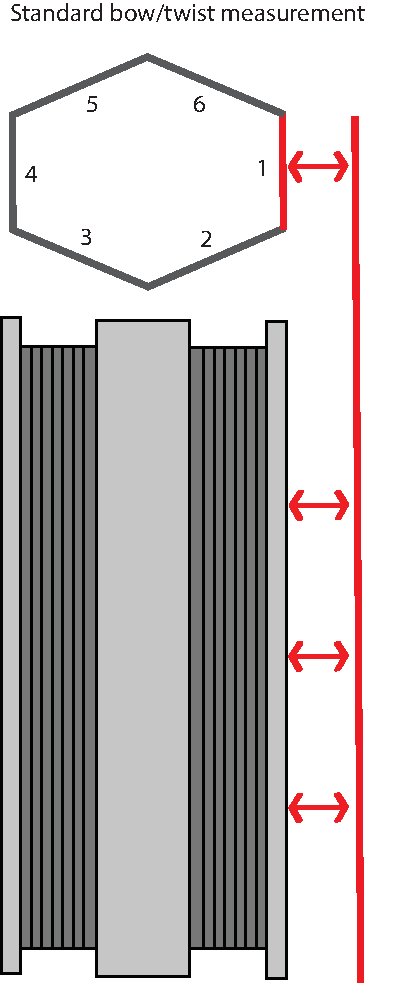
\includegraphics[width=0.3\linewidth]{std.pdf}
    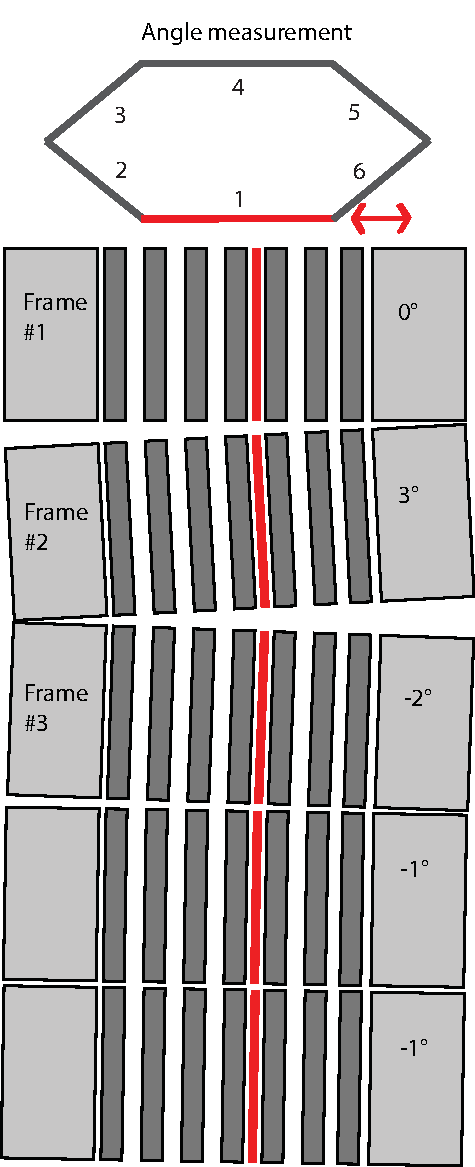
\includegraphics[width=0.31\linewidth]{angle-measurement.pdf}
    \caption{Techniques of bow measurement. Left is the standard, on the right suggested technique (DIP)}
    \label{fig:measurement_technique}
\end{figure*}

The latter approach even further limits the measurements' error, but the method still depends on the operator, who points out the measuring points - the \ac{FA}'s edge on the image, in spite of the growing automation of visual inspection, which is the current trend \cite{Guo2020}. 

The approach to utilize \ac{DIP} ensures the standardization of the evaluating process and eliminates random error. Hence all measuring points are automatically detected; the \ac{DIP} method can reach an even higher accuracy than the so-far-used. 

The given paper presents the results of the investigation of a new measuring method utilizing the \ac{DIP}. The comparison was conducted on 19 fuel assemblies of the VVER-1000  design that have covered different campaign numbers in the reactor core. The goal of the comparison was to cross the maximum \ac{FA} bow vectors obtained using both methods. The maximum bow vector refers to the highest local geometry change - perpendicular shift against the \ac{FA}'s axe. The bow vector has its length and direction. In both cases, vectors are derived from the maximum bow vector cast on the case-specific direction. Hexagonal \ac{FA} designs were measured in this study and the standard method was used on hex sides denoted as 1-3-5. The standard method's application foresees the vector's cast in the face-perpendicular direction – the bow is measured from the image's side to the \ac{FA}'s central line's face. The \ac{DIP} method calculates the bow vector component in a face-parallel direction – a shift from left to right of the full-face view (see Figure \ref{fig:measurement_technique} on the right picture where in red is marked also one side of the FA that undergoes inspection). As long as the analysis is performed on vectors, the results are fully comparable. In both cases, the maximum bow vector is calculated from three non-parallel face vectors. 

\subsection*{Data acquisition}
Fuel inspections throughout the world are focused also on anomaly detection. Each \ac{FA} design has unique criteria that allow using this kind of fuel in that reactor. It is a common correlation between used technology, required and available power output, reactor operation manner (e.g. longer or shorter campaigns), and finally used materials’ possibilities. The fuel inspection is, in this way, conducted to verify the design criteria fulfilling by the fuel.

The \ac{LWR}-type of fuel is mainly organized in fuel rods (tube-like) that are further organized in fuel assemblies. Due to this, the only possibility of tracing down the changes like sediments, enormous oxidation, defects in \ac{FA} construction, etc. is to conduct the visual inspection. Between the campaigns, there is only a small time-window during the reactor outage to conduct the fuel inspections \cite{Gabrielsson2018}. Due to time consumption, it is quite usual to select only several \ac{FA}s out of the whole core as a “representative specimen” about the behavior of all \ac{FA}s in the core. In this way, the outputs are received before the loading of the core for the next campaign, and there is the possibility to change the core pattern once the anomalies are detected.

In order to receive fast feedback about the fuel behavior, the only possibility is to conduct the inspection in the fuel storage pool environment. Due to cooling and radiation  shielding, the \ac{FA}s are submerged several meters below the coolant – usually demineralized water with a precise amount of neutron absorber as boron acid. This environment specifies the distanced mode of fuel inspection. There are 2 ways of fastening the \ac{FA} for underwater camera inspection: the \ac{FA} is placed on a rotary table; the fuel assembly is hanged. The camera system can be stationary against \ac{FA}'s face or rotating around the \ac{FA}.  The output material is a video containing the record of a whole (single) \ac{FA} side per single camera. 
In this way, the videos of all \ac{FA}’s sides are gathered. Typically, it is not possible to take an image of an entire side other than by stitching video frames together.

A natural benefit coming with this special placing of the inspected \ac{FA} is to conduct additional activities within the inspection frames to gather more information and verify another fuel design criterion. One of the most important activities are bow and twist measurements. Usually, the inspection stand (equipment) has its own gauge or specially developed measuring equipment that moves along with the camera. Nevertheless, this is an additional activity, and combining it within the mandatory visual inspection will reduce the time consumption.

The data used to develop the algorithms for bow and twist measurements were taken both in the experimental laboratory and on real nuclear fuel at the nuclear power plant. Laboratory data was prepared to simulate the \ac{NPP} conditions adequately but in a directed environment. On the laboratory dataset, it was possible to set up the processing algorithms' basic design which was then adapted for \ac{NPP} environment. 

As main problems with the real data were identified inhomogeneous lighting and light effects on the metal surface of the \ac{FA}. For this reason, the laboratory video data was gathered in different light conditions: with a light tube as well as LED-pointing lights. The used fuel rods were improved with chemically corroded surfaces reducing the natural reflectance of a clean metal surface. Due to this chemical process, random stains were developed on the fuel cladding surface what allowed to simulate various operating patterns of the fuel rods mock-ups in the reactor core. Nevertheless, the goal here was to be prepared in the best way possible before applying the designed algorithms on real \ac{FA} videos. 

The video sets of real data were taken during standard visual inspections at \ac{NPP}. Therefore, it was not possible to fully adjust the inspection to receive the best possible video samples for the \ac{DIP} designed on laboratory data. As the fuel inspection outline is prescribed, there was no possibility to do any experiment during the video grabbing.

\section{Method: Fuel assembly bow measurement}

The proposed method can be considered as a proof of concept for the construction of new, fully specialized tools for precise bow measurement or to fulfill the existing tools. The method overview includes:
\begin{enumerate}
    \item splitting of a video into frames
    \item frame analysis:
    \begin{enumerate}
        \item edge detection and smart edge detector parametrization
        \item detection of lines from edge images
        \item measurement of angles of detected lines and elimination of outliers
    \end{enumerate}
    \item analysis of frames angles:
    \begin{enumerate}
        \item identification and compensation of camera mount rotation
        \item elimination of high frequency shaking
        \item computation of real angles of rods rotation
        \item elimination of end position offset
    \end{enumerate}
    \item bow profile construction
\end{enumerate}

In the following subsections, we describe algorithms used within each step and their parametrizations. Finally, we summarize all extra requirements for video acquisition.

\subsection{Splitting of a video into frames}
A video sequence is split into separate frames where the position (=height of the recorded area relative to \ac{FA} height) is calculated from frame timestamp and camera velocity. It is necessary to ensure that camera has a constant speed over the entire processed area. Both, start and stop of the camera movement, should be set outside of the processed video sequence with suitable safety margins. 

In addition, the conversion of the analog signal to digital can cause problems with signal variance and time stability. In case of low lightning, frames become noisy and not properly labeled with a timestamp. Inaccuracies in frame timings cause blur in the collected signal which has a cumulative character in sense of bow measurement. The frames at the end of the video sequence therefore have the highest error in terms of measured distance from the expected axis.

We denote:
\begin{equation}
    F \text{ - set of frames}
\end{equation}
\begin{equation}
    f \text{ - a frame,}
\end{equation}

for each frame having a timestamp within the video sequence and an associated height on \ac{FA}.

\subsection{Frame analysis}

In the following text video resolution of about 720p is used. The parameters mentioned in the following paragraphs were not tested for other resolutions and it is highly probable that some adaptation is necessary.

\subsubsection{Preprocessing}

The goal of preprocessing steps is to get rid of data which are useless or even misleading for the \ac{FA} bow measurement. A part of each frame is negligibly affected by: 
\begin{itemize}
\item{spherical distortion (fish eye),}
\item{hardcoded texts (time, \ac{FA} identification string, ...)}

\item{black boundary}
\end{itemize}
All these affected parts can be removed from the frame without a negative effect on the processing.

For a text and black boundary elimination 25\% of the frame height and up to 10\% of width is sufficient. For prevention of large distortion caused by fish eye, we recommend normalizing the image or crop pixels with misplacement higher than 1px. For the input video, the $45^\circ$ rotated square around the frame center is used (see Figure \ref{fig:fisheye_resistant_area}). 

\begin{figure}
    \centering
    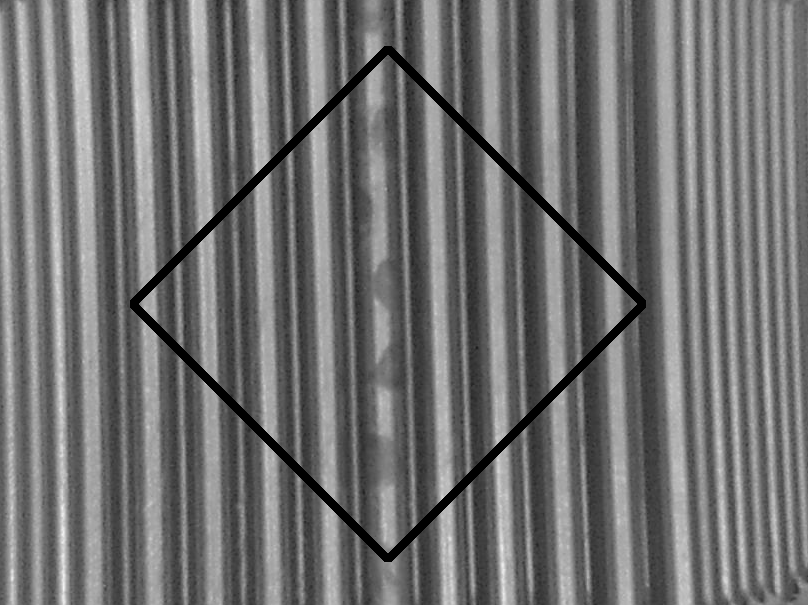
\includegraphics{central_part.png}
    \caption{Fish-eye resistant area suitable for straight line detection}
    \label{fig:fisheye_resistant_area}
\end{figure}

Next, blurring is applied on the undistorted parts of images, serving as an edge detection preprocessing step. This smooths out several minor (non-principal/noise) edges from some sharper images and prevents the edge detector to identify numerous undesired lines that do not correspond to central rods. Standard Gaussian blurring factor with a constant kernel size of 9 pixels was found to be general enough to eliminate most minor edges and keep the principal verticals, i.e.:

\begin{equation}
G(\Delta x,\Delta y,\sigma)=\frac{1}{2\pi\sigma^2}e^{-\frac{\Delta x^2+\Delta y^2}{2\sigma^2}},
\end{equation}

\begin{equation}
    I_b(x,y)=\sum_{\Delta x=-4}^4\sum_{\Delta y=-4}^{4} I(x+\Delta x, y+\Delta y) * G(\Delta x,\Delta y, 1.7),
    \label{eq:used-blur}
\end{equation}

where $G(\Delta x,\Delta y)$ is value of the gaussian factor for given $\Delta x,\Delta y$, I(x,y) is intensity of a pixel at position $x,y$ in the original image and $I_b$ is intensity in the blurred one. Equation \ref{eq:used-blur} is already parametrized by our used kernel size $=9$ and $\sigma=1.7$.

\subsubsection{Edge detector and its parametrization}

An edge detector should highlight relevant edges in the frame. Those sought edges represent rod borders, while other edges should be suppressed or eliminated by blurring.

Now, Canny edge detector \cite{Canny1986} can be used to convert preprocessed image to mask of binary edges. It has been used the already available algorithm in OpenCV library \cite{OpenCVCanny} which includes (except blur step) all steps mentioned in \cite{Canny1986} i.e.:
\begin{enumerate}
    \item Computation of intensity gradient by Sobel edge detector \cite{Sobel1968}
    \item Non-maximum suppression - edge pixels must be a local extremum in the gradient image
    \item Weak edge suppression when connectivity to strong edges is missing
\end{enumerate}
The results of this process are 1-pix wide edges (see Figure \ref{fig:angle_process} - left image). This thinness guarantees that the computation of lines will then be a stable operation. The reason is that the Hough algorithm takes each edge pixel pair to compute the orientation of the created line. In the case of wider edges (wider than 1px) one obtains a lot more edge pixels, which creates a lot more possible lines with a slightly different angle. In the case of a slightly curved line, these possible lines are constructed asymmetrically (with mean differing from 1px configuration) which can modify the computed angle of a frame. Moreover, the computation consumes much more CPU time.

The third step, weak edge suppression, of Canny's method uses two thresholds for strong/weak edge and weak edge/suppressed pixels filtration. This is extremely useful for our use case where it is necessary to preserve a stable amount of edge pixels. The intensity of pixel gradients computed by the Canny filter grows with:
\begin{itemize}
    \item{Growing oxidized layer during fuel aging}
    \item{Decreasing light intensity and growth of noisiness}
\end{itemize}
Growing oxidized layer shifts suppressed pixels towards the weak edges and therefore can be eliminated by a proper low threshold setup, while decreasing light intensity and growth of noise affect both thresholds setup. Instead of the manual setup of both thresholds, which is, in particular, subjective but also time-consuming, the process was automated by choosing proper Canny parameters by the idea of Otsu \cite{Otsu1979}. This method is based on the assumption of bimodal distribution of image pixel intensity  (corresponding to lighter and darker colors) and on choosing the best boundary between the two maxima. We propose a setup for Canny parameters based on Otsu threshold (\cite{Otsu1979} equation (19), computed by \cite{OpenCVOtsu}) in the following setting:
\begin{equation}
c_{high} = 0.3 \cdot o    
\end{equation}
\begin{equation}
c_{low} = \frac{c_{high}}{2},
\end{equation}
where $o$ denotes Otsu threshold, $c_{low}$ Canny's low threshold and $c_{high}$ Canny's high threshold. It is necessary to note that this parametrization is based on fitting our methods to the available studied dataset. It is suitable just as an entry-setup for the different dataset adaptation processes.

Successful parametrization of the Canny edge algorithm produces an edge mask presented in Figure \ref{fig:angle_process} (left image).

\begin{figure*}[hptb]
    \centering
    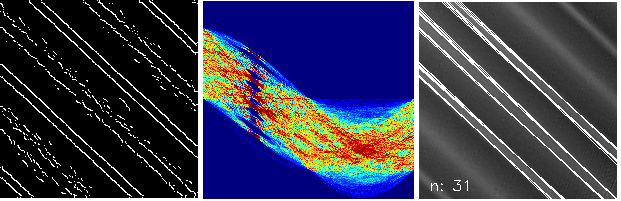
\includegraphics[width=0.95\textwidth]{angle_process-1.png}
    \caption{Illustration of the angle determination process - from Canny edges image (left),
    through Hough space (middle) to finally identified lines (right).}
    \label{fig:angle_process}
\end{figure*}

\subsubsection{Detection of lines in edge images}

The collected edges should be in the ideal case straight and oriented vertically in case of zero bow of \ac{FA}. For this reason, straight lines and their orientation are analyzed in the frames. Their angle deviation will be used afterward for bow estimation.

We propose the Hough method \cite{Hough1962, OpenCVHough}, for line detection, which transforms each edge pixel coordinates $[x,y]$ into a sinus curve in polar space (the sinus curve represents all possible straight lines going through the pixel). The sum of all sinus lines is known as the Hough space where straight lines from the edge image are represented as extrema (see Figure \ref{fig:angle_process} - middle). Moreover, each extremum is directly described by line orientation angle:
\begin{equation}
    \Theta \in (0,\pi)
\end{equation} 
and ready to use in the next step of our pipeline. The threshold (\cite{OpenCVHoughTransform}: parameter $threshold$) for preserving only relevant extrema was set to 80 pixels which is again connected to our video resolution (720p) and preprocessing frame cropping. In practice, it means that the lines with less than 80 pixels are suppressed.

Besides this threshold, Hough transformation must be also parametrized by an angle resolution (\cite{OpenCVHoughTransform}: parameter $theta$). Motivated by our target to precisely estimate \ac{FA} bow where the rotation of a frame accumulates across the whole video sequence, we propose to set up the angle resolution to $0.1^\circ$ which generates per frame bow error in the range $0-1$\textperthousand of \ac{FA} height (according to frame number).

An illustration of the entire discussed process of angle calculation is summarized in Fig. \ref{fig:angle_process}. Starting from the Canny image (left) that was based on a blurred image, the binary edges picture is transformed into Hough space within the chosen angle resolution (middle) and then identify (long-enough) straight lines based on the Hough vote size parameter (right). The resulting lines were drawn atop of the original image.

\subsubsection{Measurement of the orientation of lines and elimination of outliers}

From all angles $\Theta$ of the identified Hough lines extracted from each image, a characteristic angle $\alpha_f$ of the frame is found as a median value from all angles:

\[ \alpha_f = \Tilde{\Theta} .\]

This mitigates the error caused by several imprecisions, where short lines are filtered out and the remaining ones are aggregated into a single angle that characterizes the whole frame.
 
\subsection{Analysis of frame angles}

In this subsection, we discuss the elimination of noise caused by camera shaking and the overall lean of the camera mount, which is solved by a single procedure. All analyzed time series that are related to genuine/noise partial contributions of the angles on the fuel assembly are summarized in Fig. \ref{fig:Angles}.

\begin{figure*}
    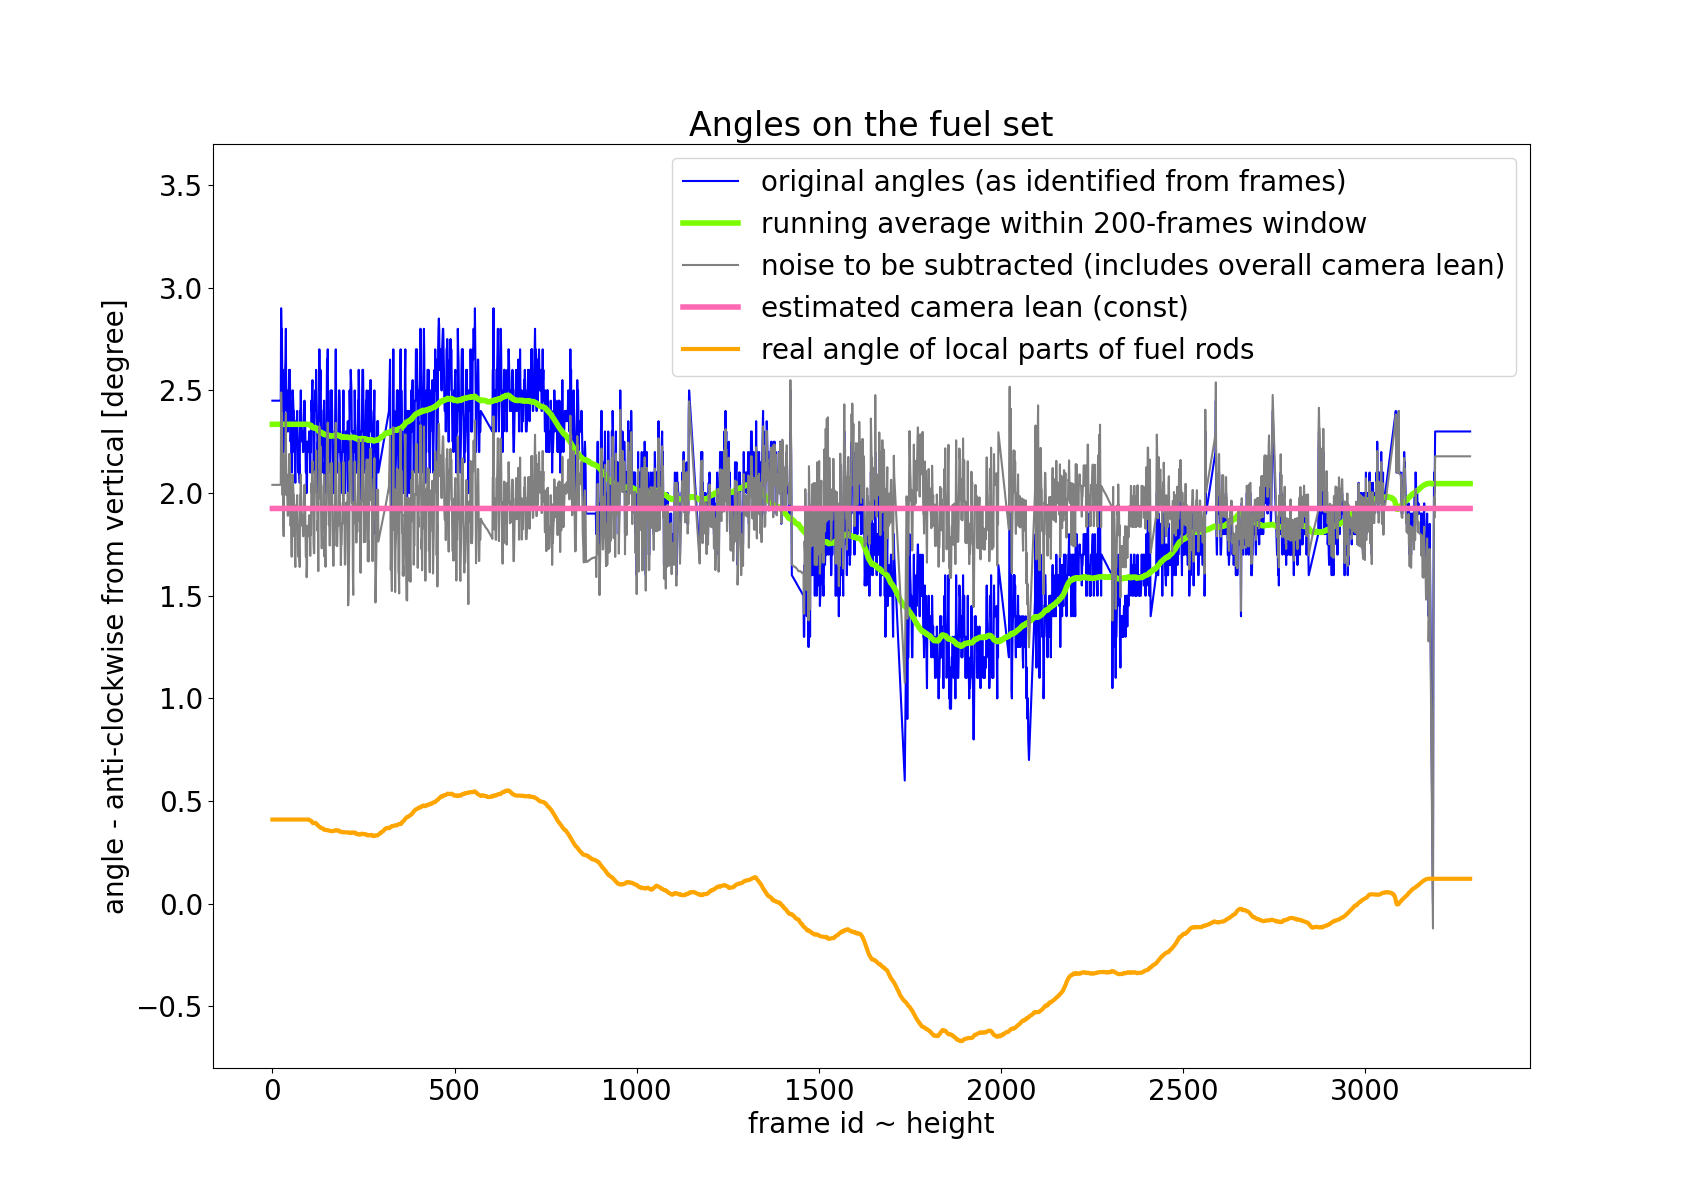
\includegraphics[width=\textwidth]{Angles.png}
    \caption{Extracted original angles from frames (blue curve), their moving average curve (MA) with 200-frames smoothing window (green curve), estimated overall lean of the camera - constant (pink straight line) and the noise series with camera lean included (gray curve) that serves to clean-up genuine signal of angles on the fuel set (orange curve).}
\label{fig:Angles}
\end{figure*}

\subsubsection{Compensation of camera mount rotation}

We assume that the global lean of camera $lean_{camera}$, which represents a deviation of the camera mount from perfect vertical, remains constant throughout the analyzed video sequence. Hence, it can be estimated by a simple average from all characteristic angles of all frames:

\begin{equation}
lean_{camera} = \frac{1}{|F|}\sum_{f \in F} \alpha_f.
\end{equation}

We note that some frames do not provide us with a recognizable angle, even after setting-up the edge detector parametrization automatically. This mainly concerns the areas where the grid is present and no vertical rods can be detected. These missing values have been interpolated by a linear interpolation scheme between the last observed and the first afterward-observed angles.

Let $\alpha_{i+1}, ... \alpha_{i+n}$ denote missing values of angles to be interpolated as:
\begin{equation}
    \alpha_{i+k} = \frac{k * \alpha_{i} + (n - k) * \alpha_{i + n + 1}}{n},
\end{equation}

where $k$ is the index of a missing frame angle starting from the last identified frame with index $i$ and $n$ is the number of missing angles in a row (in an uninterrupted sequence up to frame with index $i+n+1$).

\subsubsection{Elimination of high-frequency shaking}

To eliminate the noise caused by shaking of the unstable camera, the curve is first smoothed by $\alpha_f$. In Fig. \ref{fig:Angles}, the blue curve shows the time series of raw angles identified in one analyzed record, while the green curve represents its moving average with a smoothing window of 200 frames: 

\begin{equation}
    MA_{f_i}^{200} = \frac{1}{200}\sum_{k=-100}^{100}\alpha_{f_{i+k}}.
\end{equation}

Taking the previously estimated constant lean of the camera (pink straight line in Fig. \ref{fig:Angles}) as an undesired part of the observed angles as well, the noise angle is defined for each frame $\alpha_f^{noise}$ as the difference between the raw angle and the local value of the moving average plus the estimated camera lean: 

\[\alpha_f^{noise} = \alpha_f - MA_f^{200} + lean_{camera}, f \in F. \]

The real angle of the current part of fuel rods (with respect to vertical) is therefore estimated by subtracting the local noise from the raw angle:

\[\alpha_f^{real} = \alpha_f - \alpha_f^{noise} = MA_f^{200} - lean_{camera}, f \in F, \]

which effectively represents the running average value after the subtraction of the estimated global camera lean. The orange curve in Fig. \ref{fig:Angles} represents these finally extracted real angles, which capture local deflections of fuel rods. These angles are afterward directly used in our simple trigonometric estimation of the fuel set bow profile, as discussed later.

\subsection{From angles to fuel bow}

Once the $\alpha^{real}_f$ are computed for $\forall f \in F$ we have to transform an angle value into a frame horizontal shift. For this purpose, we use simple trigonometry:
$$
cos(\alpha_f^{real}) = \frac{\Delta x}{h_f},
$$
where $\alpha_f^{real}$ is frame real angle, $\Delta x$ is horizontal frame shift and $h_f$ is an effective frame height. The effective frame height depends on camera speed and frame rate and corresponds to number of vertical pixels by which two consecutive video frames are shifted.

Because this step acummulates the error across the video sequence, we recommend to add a procedure for double verification of computed values. The horizontal shift can also be estimated by another way. In our calibration method, we use a computation of $\Delta x$ directly from image data by minimization of this  convolution term:

$$
min_{\Delta x} -\sum_{x=0}^{W-1}I_{f_1}(x, H-1) * I_{f_2}(x + \Delta x, 0)
$$

Where $I_{f_1}$ and $I_{f_2}$ are intensities of pixels in frames $f_1$ and $f_2$ and $W$, $H$ denotes width and height of the video frames. In other words, we try to findout best position of bottom row of $f_1$ and top row of $f_2$. For this minimization we took frames for which bottom and top rows corresponds (i.e., their distance in video sequence is (e.g.) 60 frames - according to the camera speed).

Once both computational ways generate results close to each other parame\-trization for real usage is established.

\subsection{Real data application}
Processing of the \ac{NPP} data by \ac{DIP} introduced several problems in addition which had to be solved e.g. the problem of the camera stopping in the video sequence, which led to the discrepancy in the video's pixel velocity during the record, including deceleration and acceleration and the full-stop event on some grids. Besides anticipated effects like fisheye, the algorithm had to deal also with other problems like the camera's rotation and the resulting relative horizontal movement of the \ac{FA} and the camera view field (The system has a slight drift to the sides). Nevertheless, it was possible to gather enough video samples (with major or minor disadvantages) to verify the algorithms, which were in this way tested in real conditions.

The whole procedure of \ac{FA} bow measurement was constructed on already acquired datasets: video sequences, which were collected in previous years. Our approach here reveals new requirements for data and slightly changes the protocol of their acquisition for the upcoming inspections.

\section{Results}

\subsection{Standard Method} 

The commonly used method for \ac{FA} bow measurements is based on a video set in which the \ac{FA}'s side is facing left or right - perpendicular to the camera view as in Fig.\ref{fig:measurement_technique}. The camera must be moved to the side in order to see the side's edge in the center of the image. The camera goes over the height of the \ac{FA} at a constant speed. In this way, the input video is prepared in steady conditions. To evaluate the bow vector, including the \ac{FA}'s twist, it is required to perform measurements on three \ac{FA} sides for the case of hexagonal fuel. Within the standard measurement process described in this work, sides 1, 3, 5 are selected historically for measurements.

Postprocessing of the input video is based on preparing a single \ac{FA} image from the measuring film, retaining maximum accuracy in frames merging. Then, the prepared image is ready for determining the measuring points. In this way, the operator marks the red line pointing to the same construction components on each spacer grid or other standard component for the \ac{FA}'s given design. Finally, a script is run over the prepared image with red lines. The script is measuring the pixel position of the line in the image. For limiting the processing time consumption, only several points over the \ac{FA}'s height are selected as measuring points and \ac{FA}'s profile is estimated from those points. The final output is the X and Y coordinate of the bow vector for each measuring point. For better plotting, those are transformed to bow vector magnitude and its direction.

\subsection{DIP Method}

The designed \ac{SW} system for nuclear fuel deformations measurements is based on horizontal shifts of \ac{OIO} \ac{FA} face’s images. To apply the bow and twist measurements together it is necessary to know at least three side profiles on hexagonal fuel \ac{FA}’s (for a bow only, it is only two profiles). In this way, the natural result of \ac{SW} measurements is a set of two independent outputs that should be highly related, since parallel sides (in the sides numbering from 1 to 6, parallel are e.g. side 1 and side 4) should have the same bow vector magnitude, but the opposite direction (e.g. side 1 to the left and side 4 to the right). Therefore, measurements are divided into two groups, utilizing sides 1--3--5 and 2--4--6. This ”double-check” allows for better adjustment of the outputs and, in real cases, also for increased accuracy. 

The parallel sides’ issue can be seen especially on real fuel profiles. The example is shown in Fig.~\ref{fig:paralelni_strany}. As one can see, the character of profiles of parallel sides, e.g. 1 and 4, or 2 and 5, exhibits local bows directed towards the same side. However, equidistance from the zero-bow point, which should be reached in ideal conditions, is disturbed. Our opinion is that it is due to \ac{FA}’s local twist, but we do not have a ground true dataset, where we can check our hypothesis.


\begin{figure}
    \centering
    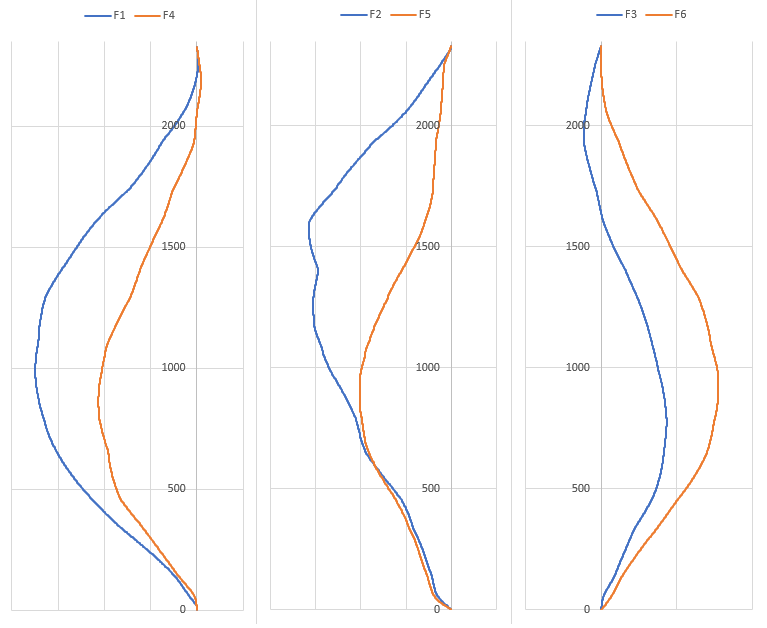
\includegraphics[width=\linewidth]{paralelni_strany.PNG}
    \caption{Whole FA sides profile – parallel sides dependency: F1 to F4, F2 to F5, and F3 to F6}
    \label{fig:paralelni_strany}
\end{figure}

The comparison of the used measuring methods shows a very good correlation between them. The \ac{DIP} measurement results are close to the standard ones obtained within the reference method. An example of such a comparison is shown in Fig.\ref{fig:B_bowdirr28}. Since the correlation between the two methods is rather high, both can be regarded as valid (due to the standard method's supposed validity). As the \ac{DIP} method provides a high density of the measured points over the \ac{FA}’s height, it also gives a better overview of the \ac{FA}’s geometrical changes along the profile. 

\begin{figure}
    \centering
    %\includegraphics[width=0.45\linewidth]{B_mag28.png}
    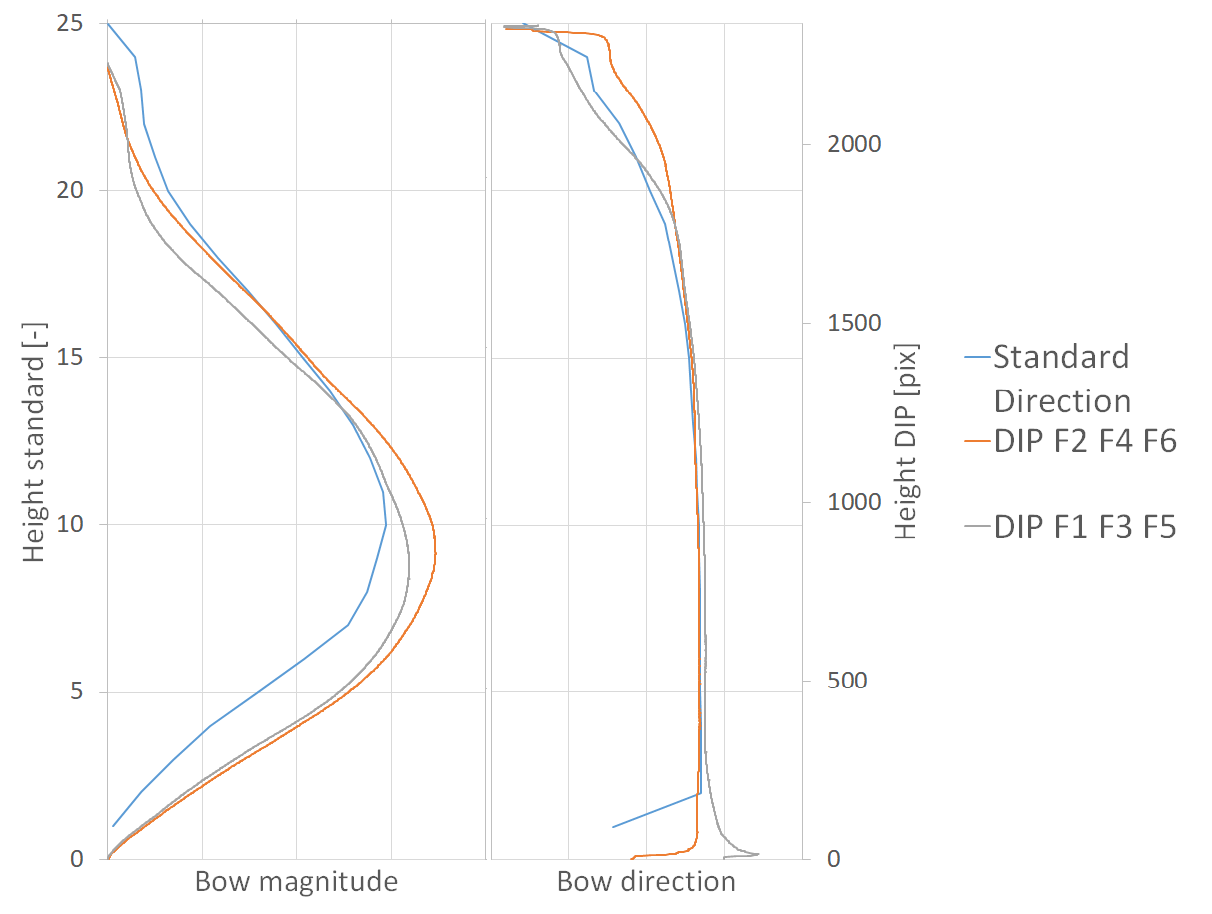
\includegraphics[width=\linewidth]{B_bowdirr28.png}
    \caption{The comparison between the standard and the DIP methods: left - bow magnitude; right - bow direction}
    \label{fig:B_bowdirr28}
\end{figure}

From the fuel inspection point of view, the essential issue is to find the maximum bow along the \ac{FA}’s height. The most bowed region could be crucial for fuel handling and for design criteria to meet. Due to this fact, the maximum bow vector was selected as the main comparison factor between the two discussed methods.

As the standard method’s measurements are usually performed on sides 1--3--5 in the case of this study, the \ac{DIP} method provides additional information about the precision of the measurements. The measurements on the complementary sides 2--4--6 - parallel to the nominal form the standard method – should provide the same results due to the method assumption. In this case, the method's overall precision can be studied as also it gives feedback about the measurements themselves – high discrepancies between the sets of measurement in the \ac{DIP} method case suggest poor algorithm performance on a particular set of data. To investigate those discrepancies, the measurements according to the standard method were performed also on sides 2--4--6 on 3 \ac{FA}s. It allowed to specify the acceptable error criterion for \ac{DIP} method. The comparison is shown in Table \ref{tab1}. One can see that the \ac{DIP} in this initial stage is not far from the standard method in this aspect. The discrepancies between the side-sets in the case of \ac{DIP} method usage per \ac{FA} still requires further investigation.

\begin{table}
\begin{tabular}{|c|c|c|}
%\cline{2-3}
\hline
Bow measurement & {magnitude diff / maximum} & {direction diff / maximum} \\ \hline
DIP method      & 2.32 \%             & 3.76 \%             \\ \hline
Standard method & 1.83 \%             & 1.94 \%             \\ \hline
\end{tabular}
\caption{
Results obtained on real fuel (3 FA's) from the comparison between standard method and \ac{SW} measurements of fuel geometrical changes. Values in the table are computed as the difference between a maximum bow computed from 1–3–5 and 2–4–6 related to the maximum allowed bow (all absolute values).}
\label{tab1}
\end{table}

To compare the described methods, the measurement's error was defined with respect to a common denominator of the maximum predicted bow. In this way, all maximum bow vector measurements have a common ground for statistical analysis. In this case, the bow vector magnitude's average has an error value of 1.81 \%, and the direction error has a value of 3.32 \%. We expect that the non-zero values can be linked with a relatively small number of analyzed \ac{FA}s  and the value will go to zero with more data included. The standard deviation of the obtained results was found to be 9.41 \% for the bow vector magnitude and 16.71 \% for the vector's direction. For reference, there is also shown the standard deviation of the standard method, which was confirmed on precisely measured \ac{FA}'s model. It is evaluated for 5 \% in bow magnitude and 6 \% in direction \cite{Mala2015}. The \ac{DIP} method has not been confronted with the gauge so far and this action is planned for the nearest future.  These results are summarized in Table \ref{tabule2}. 

\begin{table}
\begin{tabular}{|c|c|c|}
\hline
                   & Bow magnitude error & Bow direction error \\ \hline
DIP Average            & 1.81 \%             & 3.32 \%             \\ \hline
DIP Standard deviation & 9.41 \%             & 16.71 \%            \\  \hline 
STD Standard deviation & 5 \%             & 6 \%            \\ 
\hline
\end{tabular}
\caption{Error evaluation on the base of maximum predicted geometrical change.}
\label{tabule2}
\end{table}


\section{Discussion}

The methods described in this article are now discussed from two perspectives. First is the real usage of the developed methods and their possible consequences on real maintenance processes at \ac{NPP}. Second is the software complexity and precision and their possible improvements.

\subsection{Method usage and achieved unlocks}

The nuclear \ac{FA} geometrical changes are based on raw video material acquired during the \ac{FA}'s periodic visual inspection and provide us with results with sufficient accuracy. Even though the \ac{SW} developed during the presented work is at the beginning of its possible capability, the conducted studies show the inherent error smaller than 2\% for the bow's vector magnitude. As the twist is derived in a similar way as the bow vector, this assessment is also valid for the \ac{FA}'s twist quantification. Nevertheless, the issues that are still to be investigated are:

\begin{itemize}
\item Not ideally correlated results of 1-3-5 and 2-4-6 measuring sets
\item High discrepancies in the length and direction of some bow vectors
\end{itemize}

From the general point of view, there remain some higher errors in several cases, although this might be the accuracy problem of the standard methodology, which is used here as the reference (since it is a semi-visual method, where factors like perspective or image parameters can influence the outputs).

The R\&D tasks within the mentioned issues that can improve the robustness of the \ac{SW} measurements will require further testing on real fuel data and also comparing the results to multiple different standard measuring methods as references. This will be the key factor in improving the DIP framework in order to be fully prepared for real nuclear fuel inspections.

Even at this point of \ac{SW} development, however, our method is highly competitive to the standard methodology. The advantages can mainly be seen in the parallelization of the inspection's tasks – to prepare the inputs for the standard method, it is necessary to provide special video sets that take time during the inspection. The \ac{SW} application that uses the video from the \ac{FA}'s face inspection is crucially vital in the case of fuel inspection performed during a regular refueling outage. Furthermore, in the dependence of the data processing speed and the approach to inspect more than one \ac{FA}'s face at once, there is the possibility of obtaining the \ac{FA} geometry data at once after finishing the \ac{FA}'s inspection. Optionally, the \ac{FA} twist accompanies the bow on each measuring level. This widens the insight into the \ac{FA}'s behavior.  In the standard approach, the outputs are obtained in delay, as the video post-processing serves for geometry measurements. From the core reload point, the information about the \ac{FA}s geometry is vital – any fuel assembly that exceeds the geometry designed criteria cannot be reloaded to the core for the next campaign. 

A high optimization of the tasks during the fuel inspection, data elaboration, and improved accuracy (by using the \ac{SW}) and \ac{SW} processing capacities are the long-term advantages. The \ac{SW} usage will decrease the time required for the final results' preparation with the potential guarantee of preserving accuracy according to the preliminary outputs.

\subsection{Software precision and complexity}

It is necessary to mention that up to the current date, the method has not been fully adapted for GPU parallelization; therefore, real-time computations are still not achieved. The main CPU-consuming task is the Hough space computation, which depends on the number of edge pixels linearly and on the required angle precision (see Fig. \ref{fig:angles-resolution}).

\begin{figure}
    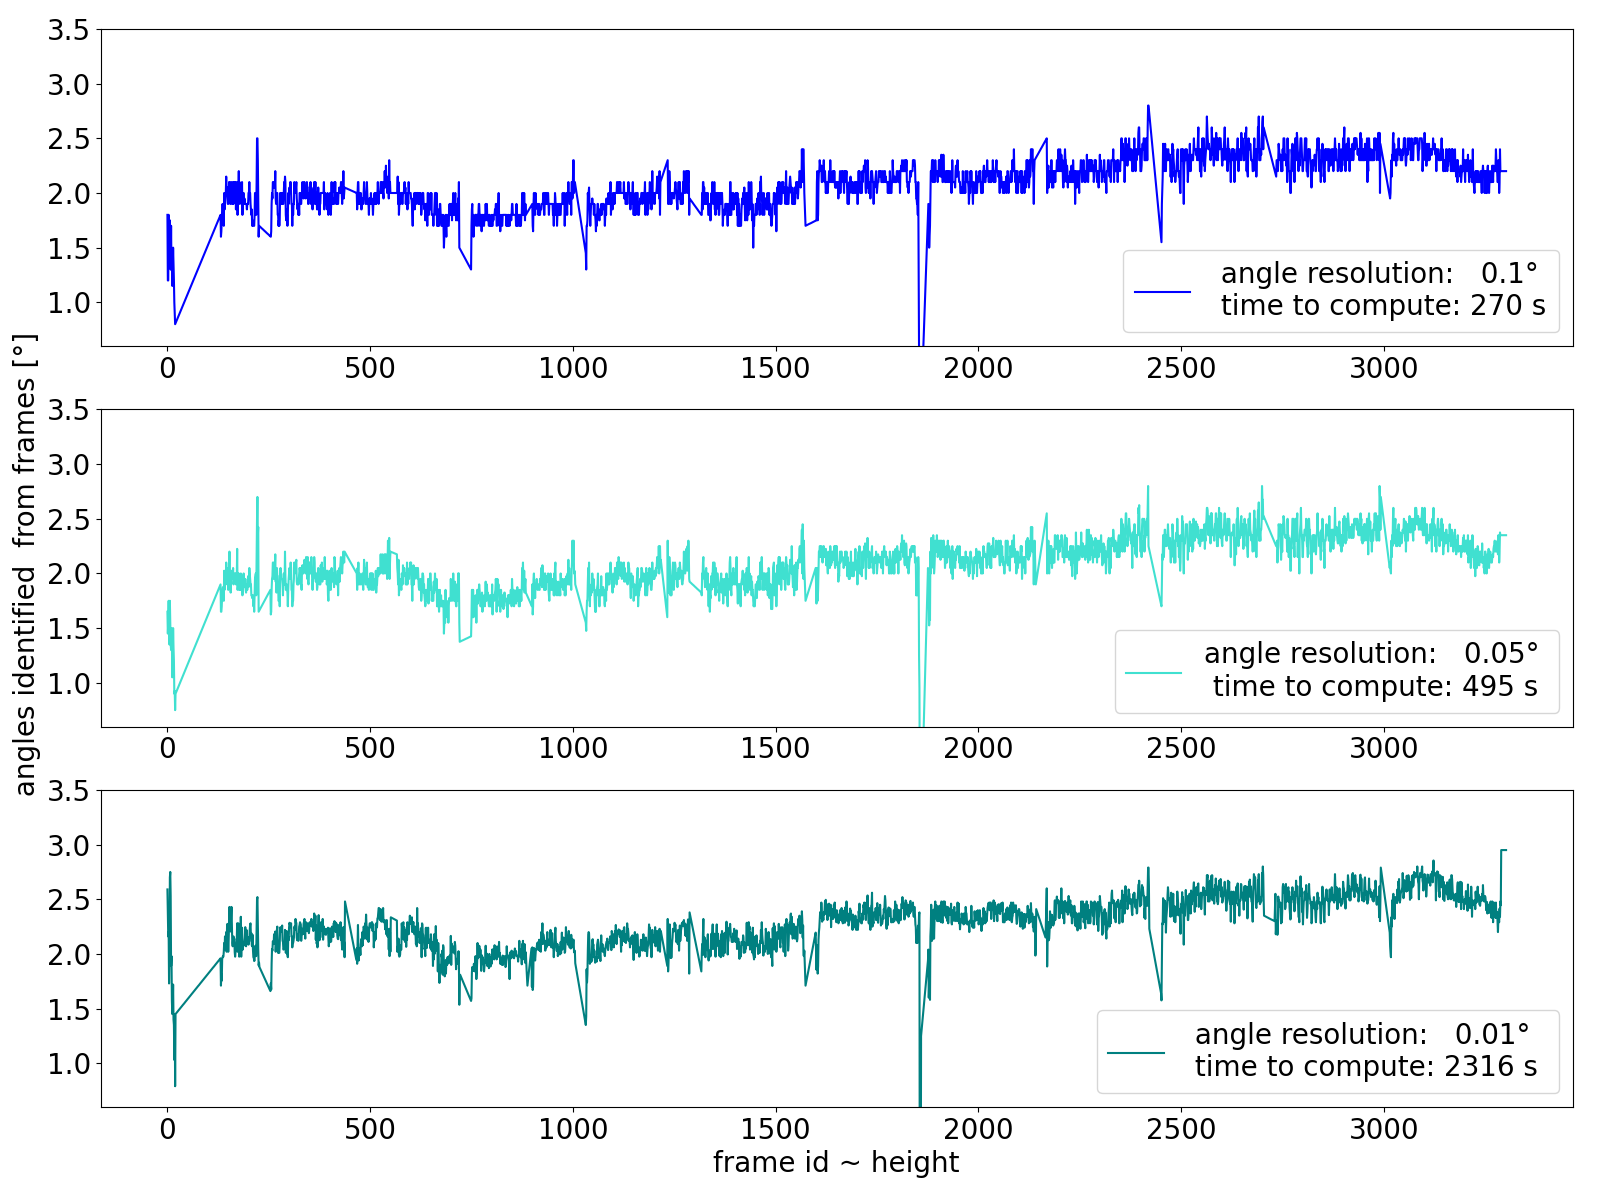
\includegraphics[width=\linewidth]{Angles-resolution.png}
    \caption{Characteristic angles of Hough lines identified from video in three different angle resolutions - 0.1$^\circ$, 0.05$^\circ$ and 0.01$^\circ$. In legends, there are noted computational times for each of the calculations to show the precision-requirements  trade-off of the calculations.}
\label{fig:angles-resolution}
\end{figure}

The precision and accuracy of the algorithm are problematic in two regards. The main problem is the cumulative error in \ac{FA} bow originating from aggregated angles. It can be concluded that the error is symmetric and the bow is realistic. However, this may not be true for different scanning devices where e.g. the frequency of shaking can interfere with video framerate and so the record would contain just positive noise angles. In case of lens distortion, it can lead to edge rotation. There are many other parameters that can lead to unrealistic bow outputs, which all can be prevented by proper calibration of the measuring device on the known object(s) (e.g. set of straight lines - plummets). 

The second regard is the hardware setup and software parametrization. The camera speed and homogeneity of illumination were already mentioned. The software design assumes that: {\label{assumption:preprocessing_frames_normalization} All frames must be clear enough to provide us with information about the characteristic angle $alpha$ of the current frame with respect to the camera. This is enabled by the visibility of central vertical rods on the \ac{FA}. Knowing typical angles on each frame then makes it possible to filter out noise from camera shaking caused by an imperfect mount.}

This assumption appeared as invalid for some spacer grids in the case of \ac{NPP} dataset because some spacer grids are too high and cover almost the whole frame at some time points; these frames (single pictures) then do not contain straight lines. The error is visible in angle charts (Fig. \ref{fig:angles-resolution}) as periodic, high amplitude, local minima (the error is the best visible around $frame\,id = [1800, 2400, 3000]$). This error is hard to fix in the dataset or acquisition process as well as in the postprocessing phase, hence it is left to use only heuristics for minimization of this effect.
The best prevention of high errors here is the reduction of angle noise i.e. unrealistic angles. For that reason, the detection mechanism used in the analysis of Hough space requires some minimal amount of lines to exist on the processed frame, otherwise, the characteristic angle is not computed.

\section{Conclusions}

In this paper, a novel method for \ac{FA} bow and twist measurements was proposed. It was compared with the currently used method at a \ac{NPP}. This method fulfills strict limits for acceptance and usage in real conditions. The achieved deviation from the current method is $1.8\%$ on average for the maximum \ac{FA} bow magnitude and $3.32\%$ for the bow direction. Our novel method is fully automatic and therefore less prone to human-based errors. In this aspect, this method overcomes the currently employed one. Moreover, the evaluation time is several times shorter than for the current method. Finally, the utilization of our novel method based on digital image processing in combination with the currently used semi-visual human-provided method makes the bow measurement more robust, which in conclusion decreases the risk of possible evaluation errors.

\vspace{6pt} 


\section*{Acknowledgements}
The presented work has been realized within Institutional Support by Ministry of Industry and Trade of the Czech Republic. We are also grateful for financial support provided by the Czech Academy of Sciences through the program Strategy AV21.

\section*{Abbreviations}
The following abbreviations are used in this manuscript:
\begin{acronym}
\acro{CVR}[CVR]{Centre of Research \v{R}e\v{z}}
\acro{FA}[FA]{nuclear fuel assembly}
\acro{OIO}[OIO]{One image overview}
\acro{SG}[SG]{Spacer grid}
\acro{IRI}[IRI]{incomplete rod insertion}
\acro{DIP}[DIP]{digital image processing}
\acro{LWR}[LWR]{Light Water Reactor}
%\acro{FME}[FME]{Foreign Materials Exclusion}
\acro{NPP}[NPP]{Nuclear Power Plant}
\acro{RCCA}[RCCA]{Rod Cluster Control Assembly}
\acro{SW}[SW]{Software}
%\acro{ROI}[ROI]{Region of interest}
\end{acronym}


%% If you have bibdatabase file and want bibtex to generate the
%% bibitems, please use
%%
 \bibliographystyle{elsarticle-num} 
 \bibliography{bibliography}
\end{document}
\endinput
%%
%% End of file `elsarticle-template-num.tex'.
